% COSC 520 Assignment 1 -- The Login Checker Problem
%
% HOW TO COMPILE (Overleaf):
%   1. On Overleaf, create a new project from the "Association for Computing
%      Machinery (ACM) - Small Standard Format Template".
%   2. Delete the template's sample .tex/.bib files.
%   3. Upload this file as main.tex, upload references.bib, and upload the
%      four PNG files from report/figures/ into a "figures" folder.
%   4. Recompile (pdfLaTeX + biber/bibtex).
%   5. Fill in the two [FILL IN] placeholders (GitHub + dataset links) and
%      the author name below before submitting.
%
% ACM copyright/journal boilerplate is intentionally suppressed below, per
% the assignment instructions.

\documentclass[acmsmall,screen=true,nonacm=true]{acmart}
\usepackage{booktabs}

% nonacm=true (above) plus the two lines below are the standard acmart way
% to suppress the ACM copyright/permission block, DOI/ISBN, and the
% "ACM Reference Format" block, per the assignment's instruction to remove
% ACM/journal/copyright information.
\setcopyright{none}
\settopmatter{printacmref=false, printccs=false}

\begin{document}

\title{The Login Checker Problem: Exact and Probabilistic Membership
  Structures at Scale}

\author{[FILL IN: Your Name]}
\affiliation{%
  \institution{University of British Columbia Okanagan, COSC 520}
  \city{Kelowna}
  \state{BC}
  \country{Canada}
}
\email{shelleybagshaw77@gmail.com}

\renewcommand{\shortauthors}{[FILL IN: Your Name]}

\begin{abstract}
Checking whether a new username collides with an existing one is a
membership-query problem that must scale to hundreds of millions of logins.
We implement, from scratch, five membership structures -- linear search,
binary search over a sorted array, a chained hash table, a Bloom filter, and
a bucketized Cuckoo filter -- and compare their theoretical and measured
build time, query time, space, and (for the two probabilistic structures)
false-positive rate. Experiments run on synthetic username sets from
$n=10^3$ to $n=10^7$ on a single machine. The exact structures agree closely
with their textbook bounds; the probabilistic filters match their published
false-positive formulas to within sampling noise, and we show that our
non-bit-packed Cuckoo implementation is \emph{not} more space-efficient than
a Bloom filter at a matched $1\%$ false-positive rate, contrary to the
folklore claim that Cuckoo filters always win below $3\%$.
\end{abstract}

\maketitle

\section{Introduction}

A login system must guarantee that every username is unique. On account
creation, the system checks whether the requested name is already stored;
on a match it must reject the request (a \emph{true positive}), and on a
genuinely new name it must accept it (a \emph{true negative}). At a scale of
hundreds of millions to a billion logins, the data structure behind this
check determines whether the operation is instantaneous or unusable.

Five approaches are compared in this report:
\begin{enumerate}
  \item \textbf{Linear search} over an unsorted list -- the naive baseline.
  \item \textbf{Binary search} over a sorted array.
  \item \textbf{Hashing} -- an exact hash table with separate chaining.
  \item \textbf{Bloom filter} -- a probabilistic set with no false negatives
    but a tunable false-positive rate, using $O(n)$ bits instead of $O(n)$
    strings.
  \item \textbf{Cuckoo filter} -- a probabilistic set that additionally
    supports deletion, storing short fingerprints instead of full keys.
\end{enumerate}

\textbf{Research question.} How do the theoretical time/space bounds of
these five structures translate into measured build time, query time, and
memory as the number of stored logins grows from $10^3$ to $10^7$, and how
closely do the two probabilistic filters match their published
false-positive formulas?

All five structures are implemented by hand (Section~\ref{sec:impl}); no
built-in \texttt{set}, \texttt{dict}, \texttt{bisect}, or third-party filter
library is used for the membership logic itself. Section~\ref{sec:complexity}
derives and justifies the complexity of each structure.
Section~\ref{sec:methodology} describes the experimental setup, and
Section~\ref{sec:results} reports the measurements. Section~\ref{sec:discussion}
compares theory against measurement, and Section~\ref{sec:threats} discusses
limitations.

\section{Data Structures and Theoretical Analysis}
\label{sec:complexity}

\subsection{Notation}

\begin{itemize}
  \item $n$: number of stored usernames.
  \item $L$: username length. In this report $L$ is treated as a small
    constant (all usernames at a given $n$ have equal length, growing only as
    $O(\log n)$), so it is folded into the implicit constant of every
    hash/compare operation unless stated otherwise.
  \item $m$: number of bits in the Bloom filter's bit array.
  \item $k$: number of hash functions (bit positions probed) in the Bloom
    filter.
  \item $p$: Bloom filter's target false-positive rate.
  \item $b$: number of buckets in the Cuckoo filter.
  \item $s$: entries (slots) per Cuckoo bucket (\texttt{bucket\_size}).
  \item $f$: Cuckoo fingerprint length in bits.
  \item $\alpha$: load factor -- for the hash table, stored items over
    bucket count; for the Cuckoo filter, occupied slots over $bs$.
  \item $R$: maximum number of Cuckoo relocation attempts per insertion
    (\texttt{max\_kicks}).
\end{itemize}

\subsection{Complexity table}

Table~\ref{tab:complexity} summarizes the bounds justified below. ``Avg''
means average case under a uniform-hashing assumption; ``Amort.'' means
amortized over a sequence of operations; ``Worst'' is an unconditional
upper bound.

\begin{table}[t]
\caption{Time and space complexity. $n$ = stored items.}
\label{tab:complexity}
\begin{tabular}{lllll}
\toprule
Structure & Build & Lookup & Delete & Space \\
\midrule
Linear search   & $O(n)$ & $O(n)$ (avg \& worst) & $O(n)$ & $O(n)$ \\
Binary search   & $O(n)$\textsuperscript{a} & $O(\log n)$ & $O(n)$ & $O(n)$ \\
Hash table      & $O(n)$ amort. & $O(1)$ avg, $O(n)$ worst & $O(1)$ avg & $O(n/\alpha)$ \\
Bloom filter    & $O(nk)$ & $O(k)$ & not supported & $O(m)=O(n\log(1/p))$ \\
Cuckoo filter   & $O(n)$ exp. amort.\textsuperscript{b} & $O(s)=O(1)$ worst & $O(s)=O(1)$ worst & $O(bsf/\alpha)$ \\
\bottomrule
\end{tabular}
\\[2pt]
\footnotesize
\textsuperscript{a}Assumes the input is already sorted (Section~\ref{sec:methodology}); building by
$n$ sequential \texttt{insert()} calls into a sorted array costs $O(n^2)$ because
each insertion shifts $O(n)$ elements. \\
\textsuperscript{b}Not unconditional: an insertion can fail if $R$ relocation
attempts are exhausted (Section~\ref{sec:cuckoo-theory}).
\end{table}

\subsubsection{Linear search}
\texttt{LinearSearchStore} appends to a Python list, $O(1)$ per insertion, so
build is $O(n)$. \texttt{contains} scans left to right and must, in the
worst case (value absent, or found at the end) inspect every element:
$O(n)$ \cite{knuth1998}. Space is $O(n)$ pointers plus the $n$ strings
themselves.

\subsubsection{Binary search}
Given an already-sorted array, \texttt{contains} halves the search interval
each iteration, giving $O(\log n)$ comparisons in the worst and average case
\cite{cormen2009}. Our \texttt{BinarySearchStore.add} performs a manual
binary search for the insertion point followed by \texttt{list.insert},
which shifts up to $O(n)$ elements; inserting $n$ items one at a time is
therefore $O(n^2)$ in the worst case. Because our synthetic generator
already returns a sorted list, the benchmark constructs the store directly
from that list (a single $O(n)$ copy, Section~\ref{sec:methodology}) rather
than paying the $O(n^2)$ incremental-insertion cost; this is stated because
the practical cost of \emph{maintaining} a sorted array under arbitrary
insertions is a well-known weakness of this approach relative to a hash
table. Deletion is symmetric to insertion: $O(n)$ for the shift.

\subsubsection{Hash table (separate chaining)}
Our \texttt{HashTable} hashes each string with a 64-bit mixed hash
(Section~\ref{sec:hashing}) and stores it in a Python list ("chain") at
bucket \texttt{hash(x) mod bucket\_count}. Under the standard uniform-hashing
assumption, each bucket holds $O(\alpha)$ elements where $\alpha=n/\text{bucket\_count}$,
so \texttt{contains} and \texttt{add} touch $O(1+\alpha)$ elements on
average \cite{cormen2009}. Doubling the table whenever $\alpha$ exceeds
\texttt{max\_load} ($0.75$ by default) keeps $\alpha=O(1)$, so lookups are
$O(1)$ average case; an adversarial input that hashes every key into one
bucket still costs $O(n)$ in the worst case. Because each resize costs
$O(n)$ but resizes happen at a geometrically shrinking frequency, building
by $n$ insertions costs $O(n)$ amortized \cite{cormen2009}. Space is the
$n$ stored strings plus $O(n/\alpha)$ bucket-array cells.

\subsubsection{Bloom filter}
\label{sec:bloom-theory}
A Bloom filter \cite{bloom1970} represents a set as an $m$-bit array.
\texttt{add} sets $k$ bit positions derived from the key; \texttt{contains}
returns \texttt{false} iff at least one of those $k$ positions is unset, so
false negatives are impossible: any bit set by a prior \texttt{add} stays
set. If a value was never inserted, each of the $k$ probed bits is,
independently under the standard idealized analysis, set with probability
$\approx 1-e^{-kn/m}$ after $n$ insertions, giving the classic false-positive
approximation \cite{bloom1970,broder2004}:
\[
p \approx \left(1-e^{-kn/m}\right)^k .
\]
Minimizing $p$ over $k$ for fixed $m,n$ gives the optimal parameters used by
our \texttt{BloomFilter.\_\_init\_\_} to size the filter for a target $p$:
\[
m = \left\lceil \frac{-n\ln p}{(\ln 2)^2} \right\rceil, \qquad
k = \max\!\left(1, \left\lfloor\frac{m}{n}\ln 2\right\rceil\right).
\]
Both \texttt{add} and \texttt{contains} touch exactly $k$ bits, so both are
$O(k)=O(\log(1/p))$ regardless of $n$; build is $O(nk)$. Space is $O(m)$ bits,
i.e., $O(n\log(1/p))$ bits, independent of the length of the stored strings.
Rather than computing $k$ independent hashes, our implementation follows the
standard double-hashing construction of Kirsch and Mitzenmacher
\cite{kirsch2006}, deriving all $k$ positions from two 64-bit hashes as
$(h_1 + i\cdot h_2)\bmod m$ for $i=0,\dots,k-1$, which is provably as
effective as $k$ independent hash functions while computing only two.

\subsubsection{Cuckoo filter}
\label{sec:cuckoo-theory}
A Cuckoo filter \cite{fan2014} stores an $f$-bit fingerprint of each key
(instead of the key itself) in one of two candidate buckets of a
bucketized cuckoo hash table \cite{pagh2004}. For key $x$ with fingerprint
$\text{fp}(x)$, the two candidate bucket indices are
\[
i_1 = h(x) \bmod b, \qquad i_2 = \bigl(i_1 \oplus h(\text{fp}(x))\bigr) \bmod b,
\]
which is symmetric: computing $i_2$ from $(i_1,\text{fp})$ or $i_1$ from
$(i_2,\text{fp})$ gives the same pair, without needing $x$ itself. Our
implementation uses subtraction modulo $b$ in place of XOR
($i_2=(h(\text{fp})-i_1)\bmod b$), which is an involution for the same
reason ($i_1=(h(\text{fp})-i_2)\bmod b$) and, unlike XOR, does not require
$b$ to be a power of two. \texttt{add} inserts the fingerprint into either
bucket if a slot is free ($O(s)$ to scan a bucket of $s$ slots); if both are
full it evicts a random entry from one bucket, recomputes that entry's
\emph{other} candidate bucket from its own fingerprint, and repeats
(``kicks''), up to $R$ times. If no free slot is found within $R$ kicks the
insertion fails; our implementation rolls back every swap performed during
the failed attempt, so a failed \texttt{add} never loses a previously
stored value. \texttt{contains} and \texttt{delete} only ever inspect the
two candidate buckets ($2s$ slots), so both are $O(s)=O(1)$ \emph{worst
case} -- unlike the hash table, no chain can grow unboundedly. Insertion is
$O(1)$ \emph{expected amortized} at load factors the structure is sized for,
but, as Fan et al.\ note, it is \textbf{not} unconditionally $O(1)$: above a
load-dependent threshold, kicks can cycle and an insertion can fail after
$R$ attempts (Table~\ref{tab:occupancy}), which is why capacity is
provisioned with headroom via a target load factor $\alpha<1$
(Section~\ref{sec:impl}).

For a target false-positive rate $\varepsilon$ and bucket size $s$, the
required fingerprint length is
\[
f \geq \left\lceil \log_2\!\frac{2s}{\varepsilon} \right\rceil
\]
\cite{fan2014}, and the total space is $b\cdot s \cdot f$ bits for
$b\approx n/(s\alpha)$ buckets, i.e., $O(nf/\alpha)$ bits.

\section{Implementation}
\label{sec:impl}

All five structures share the two-method interface
\texttt{add(value)}/\texttt{contains(value)} defined in
\texttt{base.MembershipStore} (\texttt{CuckooFilter.add} additionally
returns a boolean success flag, and both filters expose \texttt{contains}
with the same signature as the exact structures, so the benchmark harness
in Section~\ref{sec:methodology} treats all five uniformly).

\subsection{Hashing}
\label{sec:hashing}
No structure uses Python's built-in, per-process-randomized \texttt{hash()},
since that would make results non-reproducible across runs. Instead,
\texttt{hashing.py} implements FNV-1a \cite{fnv} for a base 64-bit hash and
a splitmix64-style finalizer (\texttt{derive\_hash}) to mix it and to derive
further independent-looking values from a hash and an integer index (used
for the Cuckoo filter's alternate-bucket function and the Bloom filter's
second hash). During development we measured the Cuckoo filter's
false-positive rate on our sequential \texttt{user\_000000}-style usernames
using \emph{raw} FNV-1a fingerprints (its high bits) and found it varied
between 0\% and 4\% depending on the probe-string family, because FNV-1a
mixes its low-order input bytes into its high-order output bits weakly. We
fixed this by hashing every string once through the splitmix64 finalizer
before deriving both the fingerprint and the bucket index; every family of
probe strings and stored strings then agrees with theory to within sampling
noise (Section~\ref{sec:results}). \texttt{tests/test\_hashing.py} checks
this directly by hashing 4096 sequential usernames and requiring that their
low bucket-index bits and high fingerprint bits each take at least 900
distinct values.

\subsection{Hash table}
Buckets are Python lists (\texttt{None} until first used); \texttt{add}
scans the target chain for a duplicate before appending, and the table
doubles (rehashing every entry) once size exceeds $0.75\times$bucket count.
\texttt{tests/test\_hash\_table.py} forces every value into a single bucket
(\texttt{initial\_capacity=1}, load factor disabled) to test chaining
directly, and separately tests that resizing preserves every value.

\subsection{Bloom filter}
The $m$-bit array is a \texttt{bytearray} of $\lceil m/8\rceil$ bytes
(a genuinely bit-packed layout: 8 keys' worth of bits per byte). $k$ bit
positions are derived by double hashing (Section~\ref{sec:bloom-theory}).
Tests insert 5{,}000 values and assert zero false negatives, then measure
the false-positive rate over 20{,}000 unseen probes and check it is within
statistical range of the configured target.

\subsection{Cuckoo filter}
Fingerprints are stored in one flat \texttt{array.array}, using 16-bit
cells for $f\le 16$ bits and 32-bit cells otherwise; a fingerprint of $0$
marks an empty slot, so a real fingerprint of $0$ is remapped to $1$. This
is simple and correct but \emph{not} bit-packed to the exact requested
width $f$ -- e.g., at $f=10$ bits each slot still occupies a whole 16-bit
cell in memory, which matters for the space results in
Section~\ref{sec:results}. \texttt{add} evicts uniformly at random from one
of the two candidate buckets on collision, records every displaced
fingerprint on an undo log, and rolls the log back if $R=500$ kicks are
exhausted, so \texttt{tests/test\_cuckoo\_filter.py} can force a tiny,
heavily loaded filter to fail some insertions and assert that every
\emph{accepted} value is still retrievable afterward (no false negatives),
and that fingerprint eviction chains terminate correctly by checking the
alternate-index function is its own inverse.

\section{Experimental Methodology}
\label{sec:methodology}

\textbf{Hardware/software.} Apple M4, 10 cores, 16\,GB RAM, macOS
(Darwin 24.6), CPython 3.12.

\textbf{Dataset.} Usernames are generated deterministically by
\texttt{generate\_usernames(n)}: \texttt{user\_} followed by a zero-padded
index, $0$ to $n-1$, so all $n$ names are unique and already sorted
lexicographically (which equals numeric order because the zero-padded
width is fixed for a given $n$). We tested
$n\in\{10^3,10^4,10^5,10^6,2{\times}10^6,5{\times}10^6,10^7\}$.
\textbf{Justification for $n$.} The assignment's target of $n=10^9$ would
require roughly 60\,GB just for the raw strings held by the three exact
structures (each Python string object is $\approx$49--53 bytes at this
length), which does not fit in 16\,GB of RAM; $10^7$ was the largest size
at which every structure, including the two exact structures that retain
every string, completed all trials without swapping. Because the dataset is
a pure, seedless function of $n$ (no stored randomness to lose), we publish
the generator itself plus two representative samples
(\texttt{data/samples/usernames\_1000.txt},
\texttt{data/samples/usernames\_100000.txt}) in the GitHub repository at
\textbf{[FILL IN: dataset/repo link]}, together with the one-line command
that regenerates any size exactly, including the full $n=10^7$ file used in
this report (\texttt{python -m login\_checker.dataset --count \textit{n}}).

\textbf{Queries.} For each $n$, \texttt{generate\_queries} builds
10{,}000 queries seeded by $n$: 50\% \emph{hits}, drawn uniformly at random
with replacement from the stored usernames, and 50\% \emph{misses}
(\texttt{missing\_\textit{n}\_\textit{i}}, guaranteed absent), then shuffles
the combined list. Every structure at a given $n$ receives the identical
query list, so timing differences are not explained by different inputs.
Linear search's query count is capped (e.g., 200 queries at $n=10^6$) so
that total comparisons stay bounded (Section~\ref{sec:results-linear});
its reported \emph{mean} time per query remains comparable to the other
structures.

\textbf{Measurement.} For each (structure, $n$) cell we run 5 trials at
$n\le 10^6$ and 3 trials at $n\ge 2{\times}10^6$, each on a fresh instance
built from scratch. \texttt{time.perf\_counter\_ns} brackets (a) the build
call and (b) hit and miss queries \emph{separately}, so build time never
includes query time and vice versa; CSV writing and plotting are outside
every timed region. We report the \emph{median} over trials (per
\texttt{EXPERIMENT\_PLAN.md}) to reduce sensitivity to scheduler noise, and
run 10 warm-up queries before each timed block. Peak memory of the
structure's own containers is measured with \texttt{tracemalloc} around a
fresh \texttt{factory(values)} call (a Python-level approximation: it
tracks Python object allocations, not C-level array buffers precisely
before rounding, and does not capture allocator fragmentation); the strings
in \texttt{values} already exist before that call, so for the three exact
structures that keep references to those strings we add their size
separately (\texttt{sys.getsizeof} summed over all usernames) to report a
comparable \emph{total} bytes-per-login figure. Binary search's sort/build
preprocessing is \emph{not} included in its build time, because the
generator already returns sorted data (Section~\ref{sec:complexity}); we
state this explicitly because it is the single biggest reason binary
search's build time looks better than a hash table's in
Figure~\ref{fig:build}. False positives/negatives are counted per trial by
comparing every observed answer against the exact ground truth from
\texttt{generate\_queries}.

\textbf{Accuracy experiments.} Independently of the timing benchmark,
\texttt{accuracy.py} sweeps the Bloom filter's target rate $p$ and the
Cuckoo filter's fingerprint length $f$ at fixed $n=10^5$, each measured over
200{,}000 fresh unseen probe strings, to compare measured against predicted
false-positive rates (Figure~\ref{fig:fp}); and separately inserts into
Cuckoo filters of four bucket sizes until the first insertion failure, to
measure the maximum achievable load factor (Table~\ref{tab:occupancy}).

\section{Results}
\label{sec:results}

\begin{table}[t]
\caption{Selected measurements at $n=10^6$ and $n=10^7$ (medians).
FP~rate is the fraction of miss queries reported present; FN was 0 in
every trial at every $n$.}
\label{tab:results}
\begin{tabular}{lrrrr}
\toprule
Structure & \multicolumn{2}{c}{Build time} & \multicolumn{2}{c}{Query mean (ns)} \\
 & $10^6$ & $10^7$ & $10^6$ & $10^7$ \\
\midrule
Linear   & 22.4\,ms  & --      & 6.36\,ms\textsuperscript{*} & -- \\
Binary   & 2.0\,ms   & 23.4\,ms  & 1{,}371 & 1{,}884 \\
Hash tbl.& 3.99\,s   & 38.8\,s & 1{,}660 & 1{,}729 \\
Bloom    & 2.18\,s   & 22.0\,s & 2{,}268 & 2{,}358 \\
Cuckoo   & 2.03\,s   & 21.4\,s & 1{,}908 & 2{,}121 \\
\bottomrule
\end{tabular}
\\[2pt]
\footnotesize
\textsuperscript{*}Linear search used only 200 queries at $n=10^6$
(Section~\ref{sec:methodology}) and was not run at $n=10^7$: at 10{,}000
queries it would require $O(10^{11})$ string comparisons.
\begin{tabular}{lrrrr}
& \multicolumn{2}{c}{FP rate} & \multicolumn{2}{c}{Bytes/login (total)} \\
& $10^6$ & $10^7$ & $10^6$ & $10^7$ \\
\midrule
Bloom  & 1.30\% & 1.24\% & 1.20 & 1.20 \\
Cuckoo & 0.66\% & 0.76\% & 2.32 & 2.31 \\
\bottomrule
\end{tabular}
\end{table}

\subsection{Query time}
Figure~\ref{fig:query} plots mean query time against $n$ on log-log axes,
split into the mixed workload and its hit-only/miss-only components.
Linear search grows linearly with $n$ over four orders of magnitude, as
expected; binary search grows logarithmically and remains the fastest exact
structure across the whole tested range on hits, though its miss queries
are faster than its hits (Section~\ref{sec:discussion}). The hash table,
Bloom filter, and Cuckoo filter are all flat in $n$, matching their $O(1)$
average/worst-case query bounds; the hash table is fastest of the three,
then the Cuckoo filter, then the Bloom filter, consistent with $k\approx 7$
bit probes for the Bloom filter at $p=0.01$ versus at most two bucket scans
for the Cuckoo filter and one list scan for the hash table.
\label{sec:results-linear}

\begin{figure}[t]
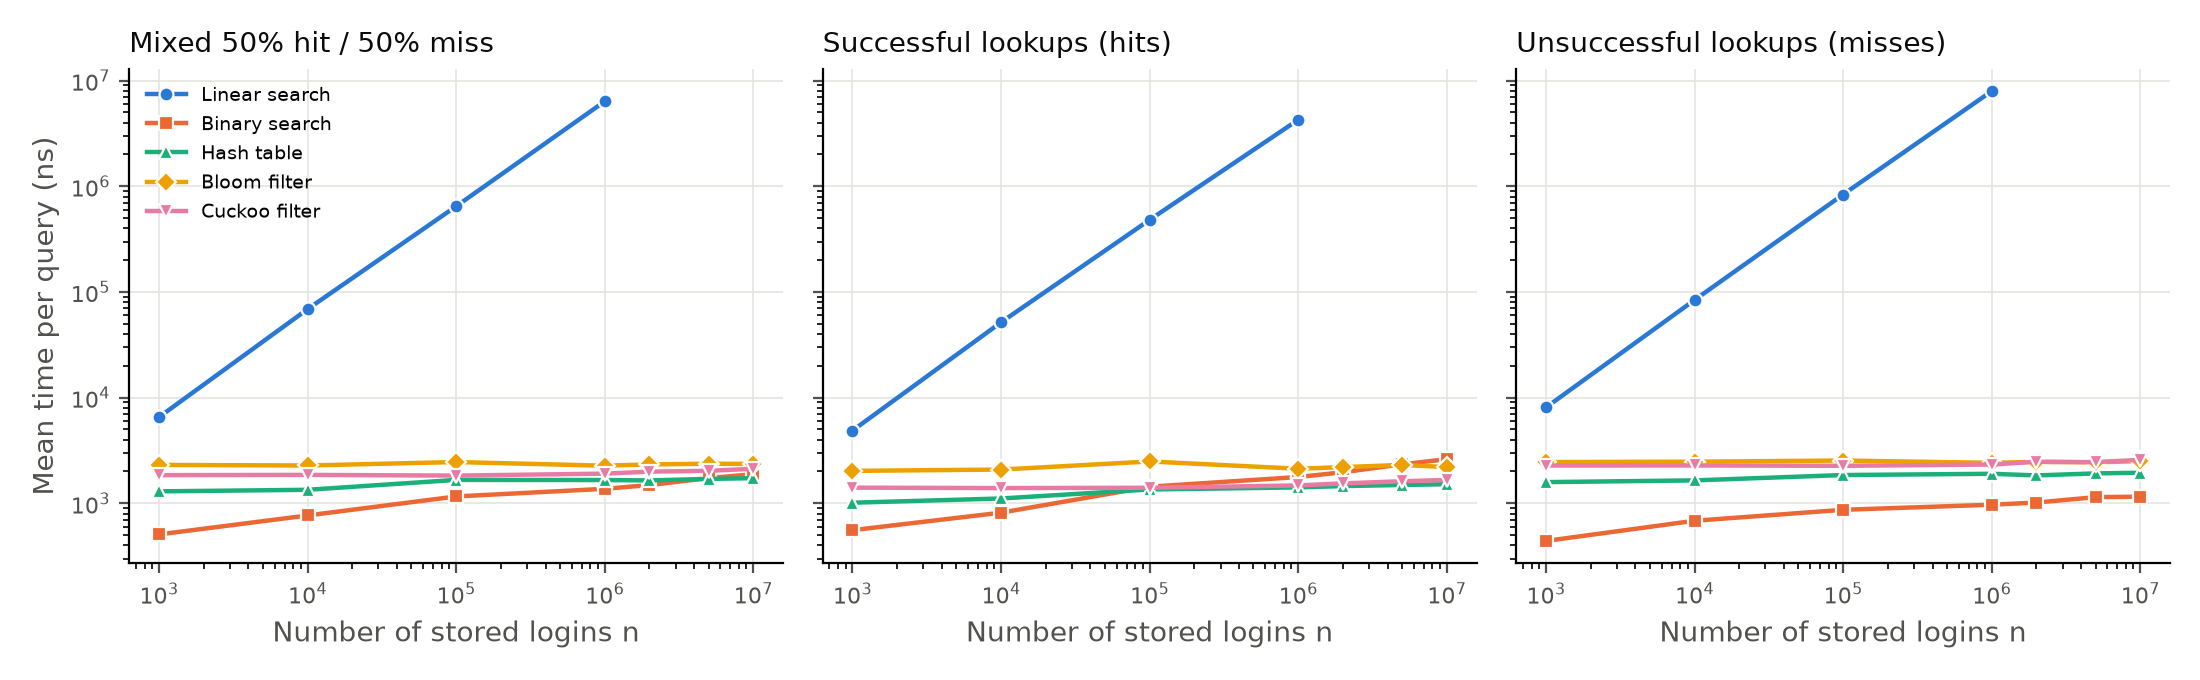
\includegraphics[width=\linewidth]{figures/query_time.png}
\caption{Mean time per query vs.\ $n$ (log-log), mixed / hit-only /
miss-only. Linear search's query count is capped above $n=10^5$
(Section~\ref{sec:methodology}).}
\label{fig:query}
\end{figure}

\subsection{Build time and space}
Figure~\ref{fig:build} shows build time. Binary search is far faster to
build than the other structures because, per
Section~\ref{sec:methodology}, its build is a single $O(n)$ copy of
already-sorted data with no per-item hashing; the hash table, Bloom filter,
and Cuckoo filter all pay an $O(n)$-with-larger-constant cost from hashing
every string, and the hash table additionally pays several $O(n)$ resize
passes. Figure~\ref{fig:memory} shows measured bytes per stored login. The
Bloom filter and Cuckoo filter use an order of magnitude less memory than
any exact structure, because they never store the strings themselves --
they use $\approx$1.2 and $\approx$2.3 bytes/login respectively, versus
$\approx$60 (array + string) for binary search and $\approx$120--130 for
the hash table's bucket/list overhead.

\begin{figure}[t]
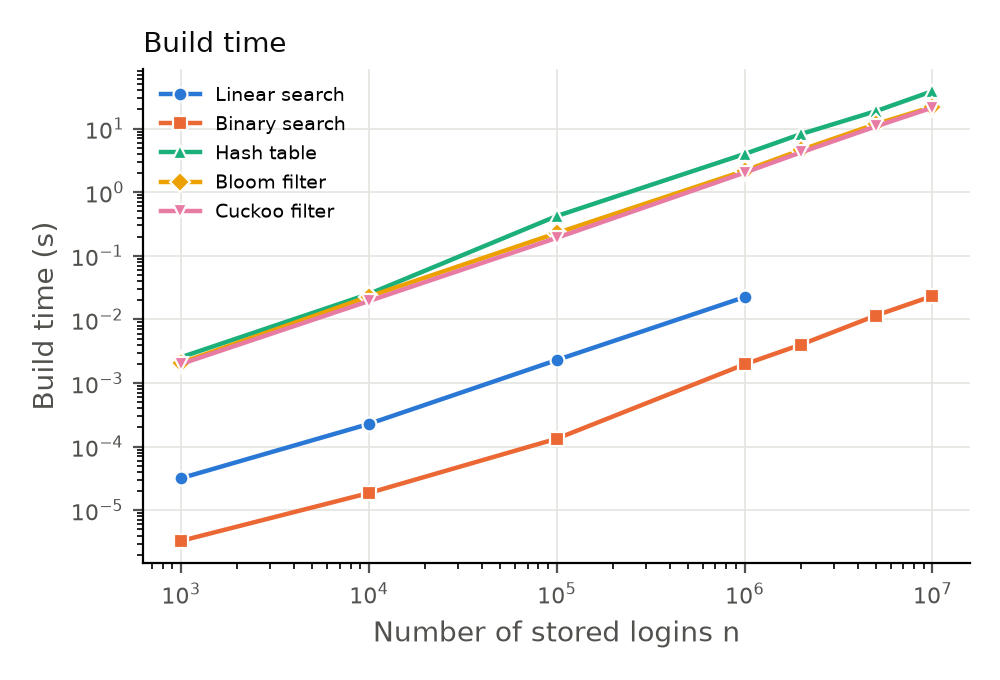
\includegraphics[width=\linewidth]{figures/build_time.png}
\caption{Total build time vs.\ $n$ (log-log).}
\label{fig:build}
\end{figure}

\begin{figure}[t]
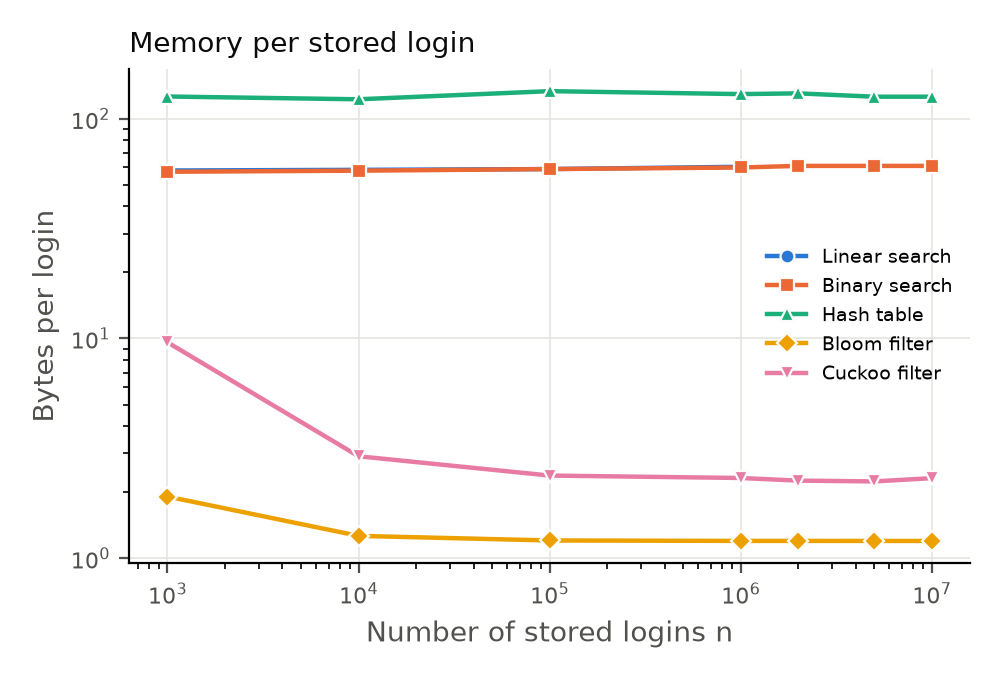
\includegraphics[width=\linewidth]{figures/memory.png}
\caption{Bytes per stored login vs.\ $n$ (log-log). Exact structures'
figures include the retained username strings.}
\label{fig:memory}
\end{figure}

\subsection{Accuracy vs.\ space}
Figure~\ref{fig:fp} sweeps each filter's space budget and compares the
measured false-positive rate over 200{,}000 unseen probes against the
formulas of Section~\ref{sec:complexity}. Both curves track their
theoretical predictions closely across three orders of magnitude in
false-positive rate ($10^{-1}$ to $10^{-4}$); no false negative was ever
observed for either filter, at any $n$, in any experiment.

\begin{figure}[t]
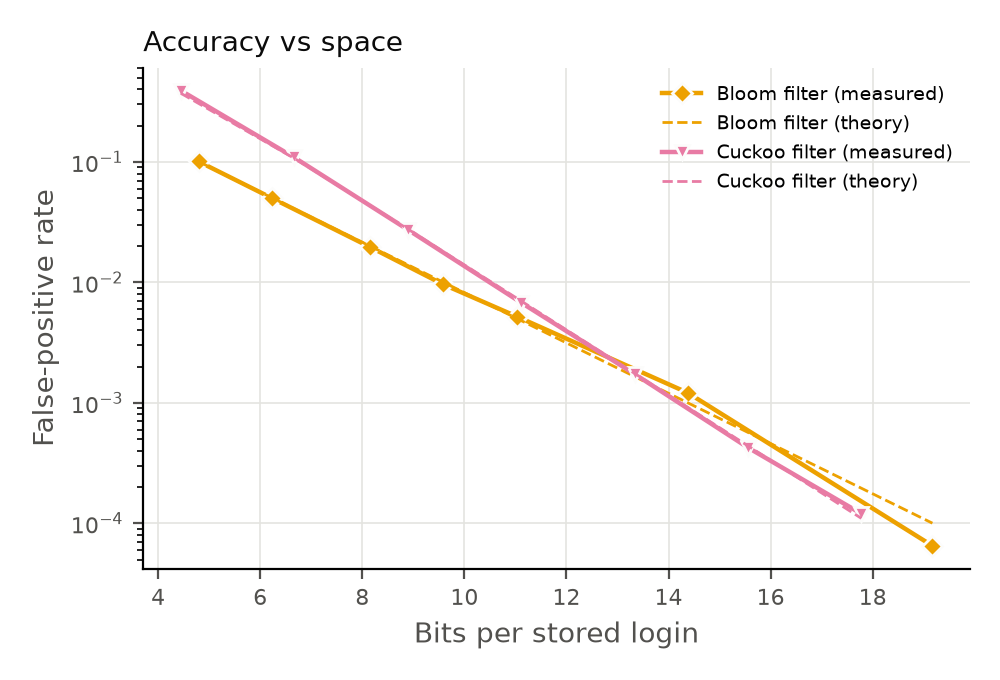
\includegraphics[width=\linewidth]{figures/false_positives.png}
\caption{Measured vs.\ predicted false-positive rate against bits per
stored login, $n=10^5$, 200{,}000 probes per point.}
\label{fig:fp}
\end{figure}

Table~\ref{tab:occupancy} shows the load factor reached before the first
Cuckoo insertion failure, for four bucket sizes at $n=10^5$
(\texttt{max\_load=1.0}, i.e., no artificial headroom): larger buckets
reach substantially higher occupancy before kicks stop finding a free slot,
matching the qualitative trend reported by Fan et al.\ \cite{fan2014}.

\begin{table}[t]
\caption{Cuckoo filter: load factor at first insertion failure, by bucket
size $s$ ($n=10^5$, no headroom).}
\label{tab:occupancy}
\begin{tabular}{lrrrr}
\toprule
$s$ & 1 & 2 & 4 & 8 \\
\midrule
Load factor & 0.523 & 0.873 & 0.966 & 0.988 \\
\bottomrule
\end{tabular}
\end{table}

\section{Discussion}
\label{sec:discussion}

\textbf{Exact structures match textbook bounds.} Linear search's query time
scales linearly with $n$ (Figure~\ref{fig:query}, left panel, a straight
line on log-log axes with slope 1), and binary search's grows
logarithmically, both as Section~\ref{sec:complexity} predicts. The hash
table, Bloom filter, and Cuckoo filter are all visibly flat, confirming
$O(1)$ average-case query time independent of $n$ across four orders of
magnitude.

\textbf{Constant factors matter more than asymptotics at this scale.}
Despite identical $O(1)$ bounds, the hash table is consistently faster per
query than both filters at every tested $n$ from $10^3$ to $10^7$: 10--42\%
faster than the Cuckoo filter and 36--78\% faster than the Bloom filter
(computed from \texttt{results/benchmark*.csv}; the gap narrows, but never
closes, as $n$ grows). The
hash table does one hash computation and one short Python-list scan; the
Bloom filter does two hash computations and $k\approx7$ modular
bit-probes into a \texttt{bytearray}; the Cuckoo filter does one hash, one
fingerprint extraction, and up to two array-scans of $s=4$ slots each,
plus (unlike the other two) an $\approx$10\% chance of missing on the
first bucket and needing the second. These per-operation constants, not
the asymptotic class, explain the ordering in Figure~\ref{fig:query}.

\textbf{Binary search's misses are faster than its hits.} A slightly
non-obvious asymmetry: Table~\ref{tab:results}-adjacent per-trial data
(\texttt{results/benchmark*.csv}) shows binary search's mean \emph{miss}
time is consistently lower than its mean \emph{hit} time (e.g.\ 969\,ns vs.\
1{,}772\,ns at $n=10^6$). This is a dataset artifact, not a general property
of binary search: every miss string (\texttt{missing\_...}) sorts before
every stored string (\texttt{user\_...}) because \texttt{'m' < 'u'}, so
every miss search takes the same short leftward path through the array,
while hits are spread uniformly across the full $\log_2 n$-depth tree. We
flag this in Section~\ref{sec:threats} rather than treat it as a property
of binary search in general.

\textbf{The Cuckoo filter is not automatically more space-efficient than
Bloom here.} A commonly repeated claim (following \cite{fan2014}) is that
Cuckoo filters use less space than Bloom filters for false-positive rates
below about 3\%. Our own numbers do not bear this out at a matched
$\approx$1\% target: the Bloom filter needs 9.6 bits/login for $p=0.01$
(Section~\ref{sec:bloom-theory}'s formula), while a Cuckoo filter at the
same false-positive rate needs a fingerprint of $f=\lceil\log_2(2s/\varepsilon)\rceil=\lceil\log_2(800)\rceil=10$
bits per entry at bucket size $s=4$, and, divided by our target load factor
$\alpha=0.9$, that is $10/0.9\approx11.1$ bits/login even in a
\emph{perfectly bit-packed} layout -- already more than the Bloom filter's
9.6 bits. The crossover Fan et al.\ report assumes load factors around
0.95--0.98 reachable with a more careful (e.g.\ semi-sorted) bucket layout;
our simple bucketized design targets $\alpha=0.9$
(Table~\ref{tab:occupancy} shows $s=4$ tops out near 0.966 \emph{before
failing}, so 0.9 leaves headroom for kicks to succeed reliably), which
pushes the crossover point below 1\%. Our \emph{measured} memory gap is
even larger than this ideal 11.1-vs-9.6 comparison: Table~\ref{tab:results}
shows $\approx$2.3 measured bytes/login (18.5 bits) for the Cuckoo filter,
because our fingerprint array uses whole 16-bit cells rather than
bit-packing to $f=10$ bits (Section~\ref{sec:impl}), while the Bloom
filter's \texttt{bytearray} is genuinely bit-packed and its measured 1.2
bytes/login (9.6 bits) matches the formula almost exactly. This is a fair
comparison of \emph{our two implementations}, but it means the
implementation effort invested in bit-packing, not just the choice of
filter family, decides which one is actually smaller in a given system.

\textbf{The Cuckoo filter's edge is deletion and worst-case lookup, not
space, in our results.} Unlike the Bloom filter, \texttt{CuckooFilter}
supports \texttt{delete} and its lookup is worst-case (not just average-case)
$O(s)$ since it never chains. At our tested false-positive rates these
were more compelling reasons to prefer it than space.

\section{Threats to Validity and Limitations}
\label{sec:threats}

\begin{itemize}
  \item \textbf{Synthetic, sequential usernames.} Real usernames are
    shorter-tailed, reused across sites, and not numerically sequential;
    our fixed-width, zero-padded names give every structure equal-length
    keys and, as discussed above, give binary search's miss queries an
    unrepresentatively short path. A more realistic generator (variable
    length, natural-language-like tokens) would be needed before
    generalizing the absolute numbers.
  \item \textbf{Single machine, single Python implementation.} All
    measurements are on one Apple M4 running CPython 3.12; results on
    other CPUs, on PyPy, or in a compiled language could shift the
    constant-factor ordering discussed in Section~\ref{sec:discussion}
    (though not the asymptotic classes).
  \item \textbf{Hash quality is empirical, not proven.} The double-hashing
    and alternate-index constructions assume close-to-uniform,
    close-to-independent hash outputs; Section~\ref{sec:hashing} describes
    a real case where an insufficiently mixed hash silently broke this
    assumption. We only tested that our mixed hash behaves well on our
    specific username families, not for arbitrary adversarial input.
  \item \textbf{tracemalloc measures Python-level allocation, not resident
    memory.} It tracks the interpreter's own allocator bookkeeping, not
    C-level buffer padding, allocator fragmentation, or copy-on-write
    sharing; the relative ordering in Figure~\ref{fig:memory} is credible,
    but the absolute bytes/login numbers should not be read as
    a hardware page-level memory measurement.
  \item \textbf{Tested sizes are $1000\times$ smaller than the assignment's
    stated target.} $n=10^7$ was the largest size that fit comfortably in
    16\,GB across all five structures (Section~\ref{sec:methodology}); the
    flatness of the $O(1)$-structures' curves out to $10^7$ is evidence for,
    but not proof of, the same behavior at $10^9$, since effects such as
    cache/TLB pressure or hash-table resize pauses could, in principle,
    change qualitatively at three more orders of magnitude.
\end{itemize}

\section{Conclusion}

Across five orders of magnitude in $n$, our from-scratch implementations
reproduce their textbook asymptotic behavior: linear search is $O(n)$,
binary search is $O(\log n)$, and the hash table, Bloom filter, and Cuckoo
filter are all flat, $O(1)$-per-query structures. At the tested scale, the
hash table gives the fastest exact queries at the cost of storing every
string, while the Bloom and Cuckoo filters cut memory by roughly an order
of magnitude in exchange for a small, tunable false-positive rate that
matched its published formula throughout our experiments, with zero
observed false negatives. Contrary to the common summary that Cuckoo
filters are simply "better than Bloom" below a few percent
false-positive rate, our matched-rate comparison shows the opposite at
$\approx$1\%: the Cuckoo filter needed more space than the Bloom filter,
both in an idealized bit-packed calculation and, more so, in our actual
non-bit-packed implementation -- a reminder that the crossover point
depends on the achievable load factor and on implementation-level packing
decisions, not on the filter family alone.

\section*{Acknowledgment and GenAI Disclosure}

Claude Code (Claude Sonnet 5, Anthropic) was used as an assistant during
this assignment. The starter repository (reference interfaces, linear and
binary search, the dataset generator's core functions, and two hash
helpers) was provided by the course. The hash table, Bloom filter, and
Cuckoo filter implementations, the extended benchmark/accuracy/plotting
scripts, and their unit tests were drafted by Claude Code from the
assignment specification and the starter interfaces, then reviewed,
run, and (where noted above, e.g.\ the FNV mixing fix) debugged against
measured results by the author. See \texttt{AI\_CONTRIBUTION\_LOG.md} in
the repository for the file-by-file breakdown and the author's own
verification notes. [FILL IN: add anything else you changed, or any
classmate/TA/web consultation, here.]

\textbf{Code:} [FILL IN: GitHub repository link] \\
\textbf{Dataset generator and sample:} [FILL IN: dataset link]

\bibliographystyle{ACM-Reference-Format}
\bibliography{references}

\end{document}
